% !TEX root = MusicFormatsCLIUserGuide.tex

% -------------------------------------------------------------------------
\chapter{MusicFormats installation modes}
% -------------------------------------------------------------------------

There is no GUI installer available yet, so users have to install the library at a lower level, sorry for that\dots.

How to install \mf\ depends on the \OS. \Linux\ users often build the software they use themselves, while those of \Windows\ and \MacOS\ are accustomed to install in much simpler ways.

Depending on the needs, users may wish to install the \MainIt{whole} \mf\ with source code and examples, or to use a \MainIt{distribution}, that contains only the \MainIt{libraries} if relevant, \CLI\ executables and documentation \pdf\ files.

The following chapters show the details.


% -------------------------------------------------------------------------
\chapter{Using a distribution}
% -------------------------------------------------------------------------

Supplied by \mf\ are tree distrubutions:
\begin{itemize}
\item \MacOS;
\item \Ubuntu;
\item \Windows.
\end{itemize}

The necessary files are found in \file{distrib}:
\begin{lstlisting}[language=Terminal]
jacquesmenu@macmini: ~/musicformats-git-dev > ls -sal distrib
total 0
0 drwxr-xr-x   5 jacquesmenu  staff  160 Feb  9 12:05 .
0 drwxr-xr-x  31 jacquesmenu  staff  992 Feb  9 10:12 ..
0 drwx------@  4 jacquesmenu  staff  128 Feb  9 13:51 macos-distrib
0 drwx------@  4 jacquesmenu  staff  128 Feb  9 16:45 ubuntu-distrib
0 drwx------@  4 jacquesmenu  staff  128 Feb  9 13:51 windows-distrib
\end{lstlisting}


% -------------------------------------------------------------------------
\section{MacOS\texttrademark\ distribution}
% -------------------------------------------------------------------------

%%%JMI\mf\ is  installable directly from the repository, since this is the environment is is developed on. Just clone the \repo\ and you will find the executables in \build{bin} and the libraries in \build{lib}.

After downloading, we get:
\begin{lstlisting}[language=Terminal]
jacquesmenu@macmini: ~/musicformats-git-dev/distrib/macos-distrib > ls -sal */*
build/bin:
total 685056
    0 drwxr-xr-x@ 25 jacquesmenu  staff       800 Feb  9 11:25 .
    0 drwxr-xr-x@  3 jacquesmenu  staff        96 Feb  9 13:51 ..
76800 -rwxr-xr-x   1 jacquesmenu  staff  38306592 Feb  9 11:25 LilyPondIssue34
76800 -rwxr-xr-x   1 jacquesmenu  staff  38309680 Feb  9 11:25 Mikrokosmos3Wandering
 9216 -rwxr-xr-x   1 jacquesmenu  staff   4314896 Feb  9 11:25 MusicAndHarmonies
 9216 -rwxr-xr-x   1 jacquesmenu  staff   4314880 Feb  9 11:25 RandomChords
 9216 -rwxr-xr-x   1 jacquesmenu  staff   4314880 Feb  9 11:25 RandomMusic
 9216 -rwxr-xr-x   1 jacquesmenu  staff   4414944 Feb  9 11:25 countnotes
17408 -rwxr-xr-x   1 jacquesmenu  staff   8313952 Feb  9 11:25 displayMusicformatsHistory
17408 -rwxr-xr-x   1 jacquesmenu  staff   8313952 Feb  9 11:25 displayMusicformatsVersion
80896 -rwxr-xr-x   1 jacquesmenu  staff  40526208 Feb  9 11:25 msdlconverter
13312 -rwxr-xr-x   1 jacquesmenu  staff   6387232 Feb  9 11:25 partsummary
 9216 -rwxr-xr-x   1 jacquesmenu  staff   4528736 Feb  9 11:25 readunrolled
64512 -rwxr-xr-x   1 jacquesmenu  staff  32618592 Feb  9 11:25 xml2brl
68608 -rwxr-xr-x   1 jacquesmenu  staff  34088624 Feb  9 11:25 xml2gmn
17408 -rwxr-xr-x   1 jacquesmenu  staff   8781984 Feb  9 11:25 xml2guido
68608 -rwxr-xr-x   1 jacquesmenu  staff  34436992 Feb  9 11:25 xml2ly
13312 -rwxr-xr-x   1 jacquesmenu  staff   6342528 Feb  9 11:25 xml2midi
60416 -rwxr-xr-x   1 jacquesmenu  staff  30426688 Feb  9 11:25 xml2xml
 9216 -rwxr-xr-x   1 jacquesmenu  staff   4657200 Feb  9 11:25 xmlclone
11264 -rwxr-xr-x   1 jacquesmenu  staff   4735296 Feb  9 11:25 xmlfactory
 9216 -rwxr-xr-x   1 jacquesmenu  staff   4504976 Feb  9 11:25 xmliter
 9216 -rwxr-xr-x   1 jacquesmenu  staff   4442496 Feb  9 11:25 xmlread
13312 -rwxr-xr-x   1 jacquesmenu  staff   6129744 Feb  9 11:25 xmltranspose
11264 -rwxr-xr-x   1 jacquesmenu  staff   4734368 Feb  9 11:25 xmlversion

documentation/IntroductionToMusicXML:
total 1672
   0 drwxr-xr-x@ 3 jacquesmenu  staff      96 Feb  9 13:51 .
   0 drwxr-xr-x@ 4 jacquesmenu  staff     128 Feb  9 13:51 ..
1672 -rw-r--r--@ 1 jacquesmenu  staff  854295 Feb  9 11:25 IntroductionToMusicXML.pdf

documentation/MusicFormatsCLIUserGuide:
total 1616
   0 drwxr-xr-x@ 3 jacquesmenu  staff      96 Feb  9 13:51 .
   0 drwxr-xr-x@ 4 jacquesmenu  staff     128 Feb  9 13:51 ..
1616 -rw-r--r--@ 1 jacquesmenu  staff  826403 Feb  9 11:25 MusicFormatsCLIUserGuide.pdf
\end{lstlisting}

\MacOS\ gets more and more stringent over time regarding security. The \OS\ part in charge of this is named \Gatekeeper. 

When installing \mf\ from the \repo\ on versions up to 10 (\Main{High Sierra}), the executables in \build{bin} are available alright.

From version 11 (\Main{Catalina}) on, though, the executables you get are not executable actually, because their developer is unknown to the \OS, and actions have to be taken for them to be usable.

The screenshot below has been made with \MacOS\ \Main{Monterey} 12.0.1 with english as the user interface language. The texts vary of course depending on the language used.

After downloading, we get:
\begin{lstlisting}[language=Terminal]
jacquesmenu@macmini: ~/Downloads/MusicFormats-for-macos/build/bin > ll
total 659992
    0 drwxr-xr-x@ 25 jacquesmenu  staff       800 Feb  5 10:17:27 2022 ./
    0 drwxr-xr-x@  4 jacquesmenu  staff       128 Feb  5 10:17:26 2022 ../
74808 -rw-r--r--@  1 jacquesmenu  staff  38301488 Feb  5 08:40:16 2022 LilyPondIssue34
74816 -rw-r--r--@  1 jacquesmenu  staff  38304608 Feb  5 08:40:16 2022 Mikrokosmos3Wandering
 8432 -rw-r--r--@  1 jacquesmenu  staff   4314896 Feb  5 08:40:16 2022 MusicAndHarmonies
 8432 -rw-r--r--@  1 jacquesmenu  staff   4314880 Feb  5 08:40:16 2022 RandomChords
 8432 -rw-r--r--@  1 jacquesmenu  staff   4314880 Feb  5 08:40:16 2022 RandomMusic
 8624 -rw-r--r--@  1 jacquesmenu  staff   4414944 Feb  5 08:40:16 2022 countnotes
16232 -rw-r--r--@  1 jacquesmenu  staff   8308416 Feb  5 08:40:18 2022 displayMusicformatsHistory
16232 -rw-r--r--@  1 jacquesmenu  staff   8308416 Feb  5 08:40:18 2022 displayMusicformatsVersion
79144 -rw-r--r--@  1 jacquesmenu  staff  40521056 Feb  5 08:40:18 2022 msdlconverter
12480 -rw-r--r--@  1 jacquesmenu  staff   6387232 Feb  5 08:40:18 2022 partsummary
 8848 -rw-r--r--@  1 jacquesmenu  staff   4528736 Feb  5 08:40:18 2022 readunrolled
63672 -rw-r--r--@  1 jacquesmenu  staff  32597328 Feb  5 08:40:20 2022 xml2brl
66544 -rw-r--r--@  1 jacquesmenu  staff  34067328 Feb  5 08:40:20 2022 xml2gmn
17160 -rw-r--r--@  1 jacquesmenu  staff   8781984 Feb  5 08:40:20 2022 xml2guido
67256 -rw-r--r--@  1 jacquesmenu  staff  34431984 Feb  5 08:40:22 2022 xml2ly
12392 -rw-r--r--@  1 jacquesmenu  staff   6342528 Feb  5 08:40:22 2022 xml2midi
59424 -rw-r--r--@  1 jacquesmenu  staff  30422064 Feb  5 08:40:22 2022 xml2xml
 9104 -rw-r--r--@  1 jacquesmenu  staff   4657200 Feb  5 08:40:22 2022 xmlclone
 9256 -rw-r--r--@  1 jacquesmenu  staff   4735296 Feb  5 08:40:22 2022 xmlfactory
 8800 -rw-r--r--@  1 jacquesmenu  staff   4504976 Feb  5 08:40:22 2022 xmliter
 8680 -rw-r--r--@  1 jacquesmenu  staff   4442496 Feb  5 08:40:24 2022 xmlread
11976 -rw-r--r--@  1 jacquesmenu  staff   6129744 Feb  5 08:40:24 2022 xmltranspose
 9248 -rw-r--r--@  1 jacquesmenu  staff   4734368 Feb  5 08:40:24 2022 xmlversion
\end{lstlisting}

These files should first made executables:
\begin{lstlisting}[language=Terminal]
jacquesmenu@macmini: ~/Downloads/MusicFormats-for-macos/build/bin > chmod +x *

jacquesmenu@macmini: ~/Downloads/MusicFormats-for-macos/build/bin > ll
total 659992
    0 drwxr-xr-x@ 25 jacquesmenu  staff       800 Feb  5 10:17:27 2022 ./
    0 drwxr-xr-x@  4 jacquesmenu  staff       128 Feb  5 10:17:26 2022 ../
74808 -rwxr-xr-x@  1 jacquesmenu  staff  38301488 Feb  5 08:40:16 2022 LilyPondIssue34*
74816 -rwxr-xr-x@  1 jacquesmenu  staff  38304608 Feb  5 08:40:16 2022 Mikrokosmos3Wandering*
 8432 -rwxr-xr-x@  1 jacquesmenu  staff   4314896 Feb  5 08:40:16 2022 MusicAndHarmonies*
 8432 -rwxr-xr-x@  1 jacquesmenu  staff   4314880 Feb  5 08:40:16 2022 RandomChords*
 8432 -rwxr-xr-x@  1 jacquesmenu  staff   4314880 Feb  5 08:40:16 2022 RandomMusic*
 8624 -rwxr-xr-x@  1 jacquesmenu  staff   4414944 Feb  5 08:40:16 2022 countnotes*
16232 -rwxr-xr-x@  1 jacquesmenu  staff   8308416 Feb  5 08:40:18 2022 displayMusicformatsHistory*
16232 -rwxr-xr-x@  1 jacquesmenu  staff   8308416 Feb  5 08:40:18 2022 displayMusicformatsVersion*
79144 -rwxr-xr-x@  1 jacquesmenu  staff  40521056 Feb  5 08:40:18 2022 msdlconverter*
12480 -rwxr-xr-x@  1 jacquesmenu  staff   6387232 Feb  5 08:40:18 2022 partsummary*
 8848 -rwxr-xr-x@  1 jacquesmenu  staff   4528736 Feb  5 08:40:18 2022 readunrolled*
63672 -rwxr-xr-x@  1 jacquesmenu  staff  32597328 Feb  5 08:40:20 2022 xml2brl*
66544 -rwxr-xr-x@  1 jacquesmenu  staff  34067328 Feb  5 08:40:20 2022 xml2gmn*
17160 -rwxr-xr-x@  1 jacquesmenu  staff   8781984 Feb  5 08:40:20 2022 xml2guido*
67256 -rwxr-xr-x@  1 jacquesmenu  staff  34431984 Feb  5 08:40:22 2022 xml2ly*
12392 -rwxr-xr-x@  1 jacquesmenu  staff   6342528 Feb  5 08:40:22 2022 xml2midi*
59424 -rwxr-xr-x@  1 jacquesmenu  staff  30422064 Feb  5 08:40:22 2022 xml2xml*
 9104 -rwxr-xr-x@  1 jacquesmenu  staff   4657200 Feb  5 08:40:22 2022 xmlclone*
 9256 -rwxr-xr-x@  1 jacquesmenu  staff   4735296 Feb  5 08:40:22 2022 xmlfactory*
 8800 -rwxr-xr-x@  1 jacquesmenu  staff   4504976 Feb  5 08:40:22 2022 xmliter*
 8680 -rwxr-xr-x@  1 jacquesmenu  staff   4442496 Feb  5 08:40:24 2022 xmlread*
11976 -rwxr-xr-x@  1 jacquesmenu  staff   6129744 Feb  5 08:40:24 2022 xmltranspose*
 9248 -rwxr-xr-x@  1 jacquesmenu  staff   4734368 Feb  5 08:40:24 2022 xmlversion*
\end{lstlisting}

Then, when launching one of these executables such as:
\begin{lstlisting}[language=Terminal]
jacquesmenu@macmini > ./xml2ly 
\end{lstlisting}
we get a alert telling that it cannot be opened, because the developper is not known to the \OS:\\
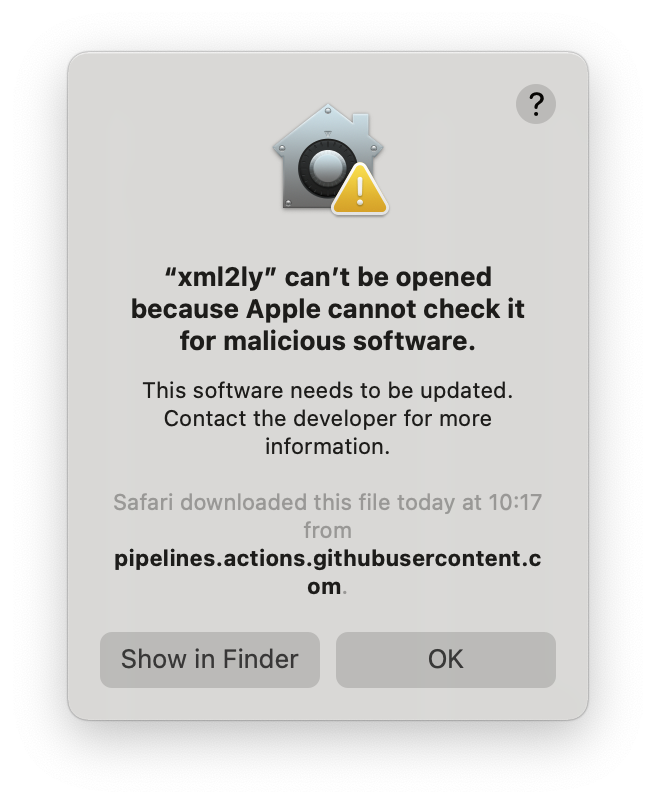
\includegraphics[scale=0.5]{../graphics/MacOSMaliciousSoftwareAlert.png}

Clicking in either buttons in this dialog kill the process:
\begin{lstlisting}[language=Terminal]
Killed: 9
\end{lstlisting}

The trouble is that these executables are in {\it \quarantine} by default. To make them usable, they have to quit quarantine, which is done by removing one of their attributes:
\begin{lstlisting}[language=Terminal]
xattr -d com.apple.quarantine *
\end{lstlisting}
%codesign --sign - --force --deep %%%JMI not necessary

From then on, the \mf\ executables can be used seamlessly on the given machine.

Having to perform the preceding task for each executable is the price to pay for security. And it has to be perfomed again when installing new versions\dots


%The way to go ahead is, right after you got that message, is to:
%\begin{itemize}
%\item  open \MainIt{System Preferences}, choose the \MainIt{Security \& Privacy} tab, and there click on the \MainIt{General button};
%
%\item click on the lock at the bottom left of the dialog to make changes:\\
%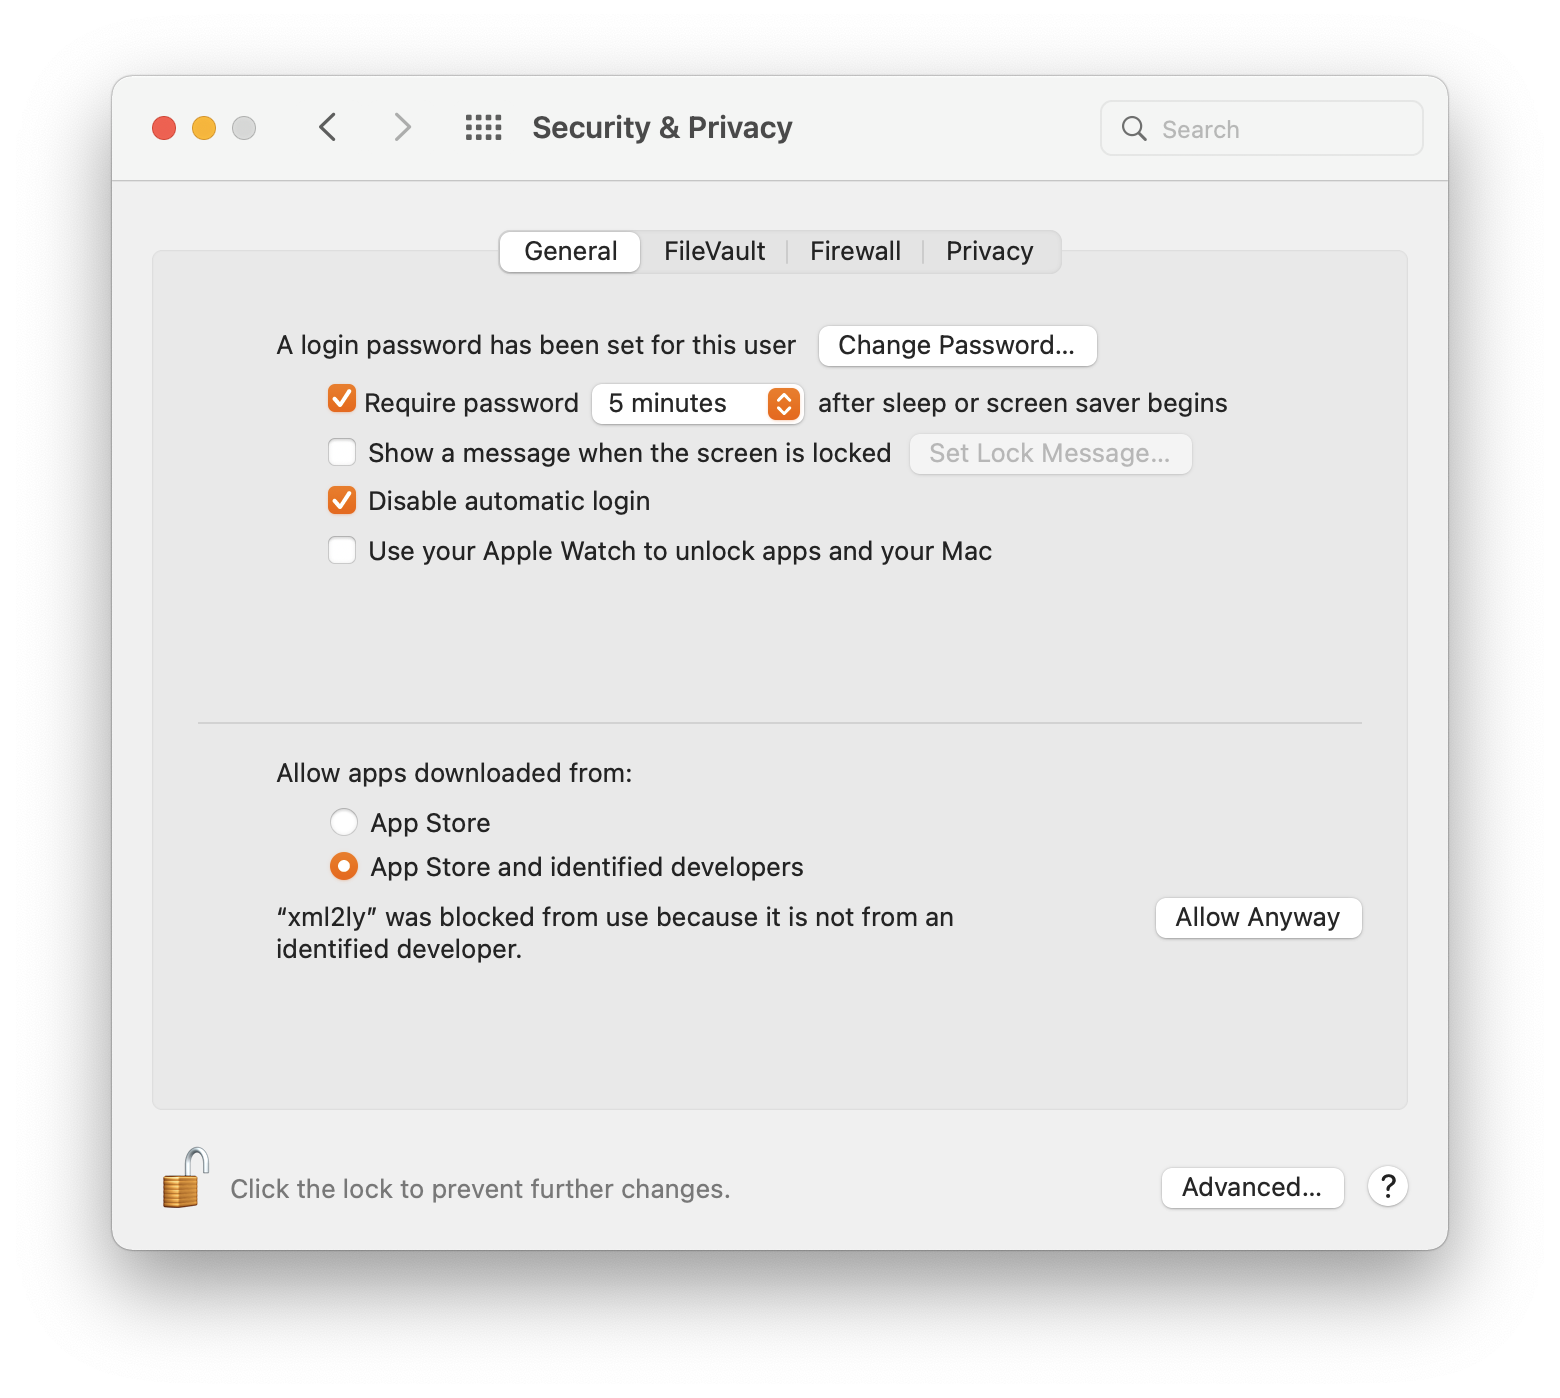
\includegraphics[scale=0.5]{../graphics/MacOSAllowAnyway.png}
%
%\item click on the \MainIt{Allow Anyway} button.
%%%%JMI sudo spctl --master-disable to create a Anywhere radio button
%%jacquesmenu@macmini > spctl --status
%%assessments enabled
%
%\end{itemize}
%
%Re-execute the executable from the command line. This pops-up a dialog to confirm you actually want to use this software:\\
%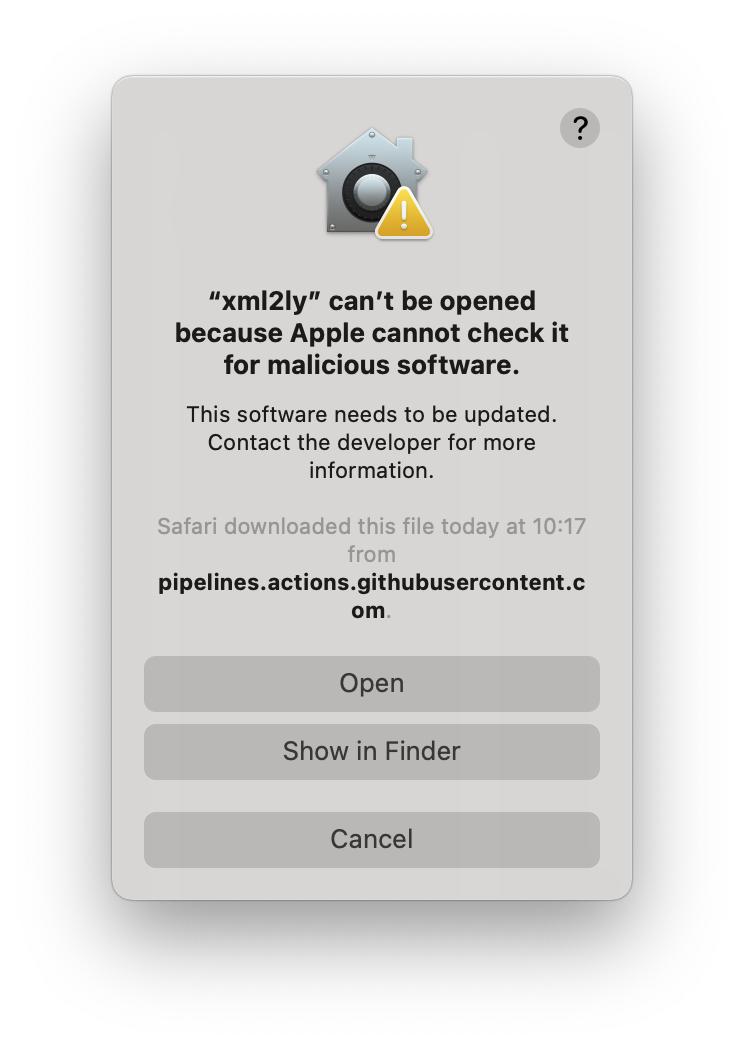
\includegraphics[scale=0.5]{../graphics/MacOSConfirmOpening.png}
%
%Click on the \MainIt{Open} button to register the executable in \Gatekeeper\ and go ahead.


% -------------------------------------------------------------------------
\section{Ubuntu distribution}
% -------------------------------------------------------------------------

After downloading, we get:
\begin{lstlisting}[language=Terminal]
jacquesmenu@macmini: ~/musicformats-git-dev/distrib/ubuntu-distrib > ls -sal */*
build/bin:
total 2264
  0 drwxr-xr-x@ 25 jacquesmenu  staff     800 Feb  9 16:45 .
  0 drwxr-xr-x@  4 jacquesmenu  staff     128 Feb  9 16:45 ..
 80 -rw-r--r--@  1 jacquesmenu  staff   39256 Feb  9 13:40 LilyPondIssue34
 80 -rw-r--r--@  1 jacquesmenu  staff   39288 Feb  9 13:40 Mikrokosmos3Wandering
 96 -rw-r--r--@  1 jacquesmenu  staff   47224 Feb  9 13:40 MusicAndHarmonies
 96 -rw-r--r--@  1 jacquesmenu  staff   47216 Feb  9 13:40 RandomChords
 96 -rw-r--r--@  1 jacquesmenu  staff   47216 Feb  9 13:40 RandomMusic
 72 -rw-r--r--@  1 jacquesmenu  staff   33800 Feb  9 13:40 countnotes
 40 -rw-r--r--@  1 jacquesmenu  staff   17648 Feb  9 13:40 displayMusicformatsHistory
 40 -rw-r--r--@  1 jacquesmenu  staff   17648 Feb  9 13:40 displayMusicformatsVersion
104 -rw-r--r--@  1 jacquesmenu  staff   49760 Feb  9 13:40 msdlconverter
544 -rw-r--r--@  1 jacquesmenu  staff  275976 Feb  9 13:40 partsummary
 88 -rw-r--r--@  1 jacquesmenu  staff   43720 Feb  9 13:40 readunrolled
 80 -rw-r--r--@  1 jacquesmenu  staff   39200 Feb  9 13:40 xml2brl
 88 -rw-r--r--@  1 jacquesmenu  staff   43336 Feb  9 13:40 xml2gmn
 48 -rw-r--r--@  1 jacquesmenu  staff   23112 Feb  9 13:40 xml2guido
 80 -rw-r--r--@  1 jacquesmenu  staff   39056 Feb  9 13:40 xml2ly
 88 -rw-r--r--@  1 jacquesmenu  staff   42880 Feb  9 13:40 xml2midi
 88 -rw-r--r--@  1 jacquesmenu  staff   43344 Feb  9 13:40 xml2xml
 88 -rw-r--r--@  1 jacquesmenu  staff   43368 Feb  9 13:40 xmlclone
 48 -rw-r--r--@  1 jacquesmenu  staff   22616 Feb  9 13:40 xmlfactory
168 -rw-r--r--@  1 jacquesmenu  staff   83488 Feb  9 13:40 xmliter
 56 -rw-r--r--@  1 jacquesmenu  staff   28424 Feb  9 13:40 xmlread
 56 -rw-r--r--@  1 jacquesmenu  staff   28656 Feb  9 13:40 xmltranspose
 40 -rw-r--r--@  1 jacquesmenu  staff   17360 Feb  9 13:40 xmlversion

build/lib:
total 159744
     0 drwxr-xr-x@ 4 jacquesmenu  staff       128 Feb  9 16:45 .
     0 drwxr-xr-x@ 4 jacquesmenu  staff       128 Feb  9 16:45 ..
113664 -rw-r--r--@ 1 jacquesmenu  staff  57941702 Feb  9 13:40 libmusicxml2.a
 46080 -rw-r--r--@ 1 jacquesmenu  staff  22806336 Feb  9 13:40 libmusicxml2.so

documentation/IntroductionToMusicXML:
total 1672
   0 drwxr-xr-x@ 3 jacquesmenu  staff      96 Feb  9 16:45 .
   0 drwxr-xr-x@ 4 jacquesmenu  staff     128 Feb  9 16:45 ..
1672 -rw-r--r--@ 1 jacquesmenu  staff  854295 Feb  9 13:40 IntroductionToMusicXML.pdf

documentation/MusicFormatsCLIUserGuide:
total 1616
   0 drwxr-xr-x@ 3 jacquesmenu  staff      96 Feb  9 16:45 .
   0 drwxr-xr-x@ 4 jacquesmenu  staff     128 Feb  9 16:45 ..
1616 -rw-r--r--@ 1 jacquesmenu  staff  826403 Feb  9 13:40 MusicFormatsCLIUserGuide.pdf
\end{lstlisting}


% -------------------------------------------------------------------------
\section{Windows\texttrademark\ distribution}
% -------------------------------------------------------------------------

After downloading, we get:
\begin{lstlisting}[language=Terminal]
jacquesmenu@macmini: ~/musicformats-git-dev/distrib/windows-distrib > ls -sal */*
build/bin:
total 1192
  0 drwxr-xr-x@ 25 jacquesmenu  staff    800 Feb  9 13:51 .
  0 drwxr-xr-x@  4 jacquesmenu  staff    128 Feb  9 13:51 ..
 64 -rw-r--r--@  1 jacquesmenu  staff  30208 Feb  9 12:03 LilyPondIssue34.exe
 64 -rw-r--r--@  1 jacquesmenu  staff  30720 Feb  9 12:03 Mikrokosmos3Wandering.exe
 56 -rw-r--r--@  1 jacquesmenu  staff  26112 Feb  9 12:03 MusicAndHarmonies.exe
 56 -rw-r--r--@  1 jacquesmenu  staff  25088 Feb  9 12:03 RandomChords.exe
 56 -rw-r--r--@  1 jacquesmenu  staff  25088 Feb  9 12:03 RandomMusic.exe
 32 -rw-r--r--@  1 jacquesmenu  staff  14848 Feb  9 12:03 countnotes.exe
 24 -rw-r--r--@  1 jacquesmenu  staff  10752 Feb  9 12:03 displayMusicformatsHistory.exe
 24 -rw-r--r--@  1 jacquesmenu  staff  10752 Feb  9 12:03 displayMusicformatsVersion.exe
 72 -rw-r--r--@  1 jacquesmenu  staff  35328 Feb  9 12:03 msdlconverter.exe
112 -rw-r--r--@  1 jacquesmenu  staff  56832 Feb  9 12:03 partsummary.exe
 40 -rw-r--r--@  1 jacquesmenu  staff  18432 Feb  9 12:03 readunrolled.exe
 64 -rw-r--r--@  1 jacquesmenu  staff  32768 Feb  9 12:03 xml2brl.exe
 72 -rw-r--r--@  1 jacquesmenu  staff  33280 Feb  9 12:03 xml2gmn.exe
 64 -rw-r--r--@  1 jacquesmenu  staff  29184 Feb  9 12:03 xml2guido.exe
 64 -rw-r--r--@  1 jacquesmenu  staff  32768 Feb  9 12:03 xml2ly.exe
 40 -rw-r--r--@  1 jacquesmenu  staff  17920 Feb  9 12:03 xml2midi.exe
 72 -rw-r--r--@  1 jacquesmenu  staff  33280 Feb  9 12:03 xml2xml.exe
 32 -rw-r--r--@  1 jacquesmenu  staff  14848 Feb  9 12:03 xmlclone.exe
 32 -rw-r--r--@  1 jacquesmenu  staff  15360 Feb  9 12:03 xmlfactory.exe
 40 -rw-r--r--@  1 jacquesmenu  staff  19456 Feb  9 12:03 xmliter.exe
 56 -rw-r--r--@  1 jacquesmenu  staff  27136 Feb  9 12:03 xmlread.exe
 32 -rw-r--r--@  1 jacquesmenu  staff  14848 Feb  9 12:03 xmltranspose.exe
 24 -rw-r--r--@  1 jacquesmenu  staff  12288 Feb  9 12:03 xmlversion.exe

build/lib:
total 38912
    0 drwxr-xr-x@ 4 jacquesmenu  staff       128 Feb  9 13:51 .
    0 drwxr-xr-x@ 4 jacquesmenu  staff       128 Feb  9 13:51 ..
15360 -rw-r--r--@ 1 jacquesmenu  staff   7517760 Feb  9 12:03 musicxml2.exp
23552 -rw-r--r--@ 1 jacquesmenu  staff  11598816 Feb  9 12:03 musicxml2.lib

documentation/IntroductionToMusicXML:
total 1672
   0 drwxr-xr-x@ 3 jacquesmenu  staff      96 Feb  9 13:51 .
   0 drwxr-xr-x@ 4 jacquesmenu  staff     128 Feb  9 13:51 ..
1672 -rw-r--r--@ 1 jacquesmenu  staff  854295 Feb  9 12:03 IntroductionToMusicXML.pdf

documentation/MusicFormatsCLIUserGuide:
total 1616
   0 drwxr-xr-x@ 3 jacquesmenu  staff      96 Feb  9 13:51 .
   0 drwxr-xr-x@ 4 jacquesmenu  staff     128 Feb  9 13:51 ..
1616 -rw-r--r--@ 1 jacquesmenu  staff  826403 Feb  9 12:03 MusicFormatsCLIUserGuide.pdf
\end{lstlisting}


% -------------------------------------------------------------------------
\chapter{Full installation}
% -------------------------------------------------------------------------

% -------------------------------------------------------------------------
\section{Cloning the repository}
% -------------------------------------------------------------------------

The library should be cloned locally, on the user's machine, with the command below. This creates a local copy (a \MainIt{clone} in \git's terminology) of the repository's contents, named here \code{musicformats_local_clone}:
\begin{lstlisting}[language=Terminal]
jacquesmenu@macmini: ~ > git clone https://github.com/jacques-menu/musicformats.git musicformats_local_clone
Cloning into 'musicformats_local_clone'...
remote: Enumerating objects: 20619, done.
remote: Counting objects: 100% (15175/15175), done.
remote: Compressing objects: 100% (7546/7546), done.
remote: Total 20619 (delta 13189), reused 9420 (delta 7560), pack-reused 5444
Receiving objects: 100% (20619/20619), 107.32 MiB | 11.14 MiB/s, done.
Resolving deltas: 100% (15569/15569), done.
\end{lstlisting}

More precisely, the local copy is that of the \MainIt{default branch}, which is a stable one, i.e. you can use is safely. It contains:
\begin{lstlisting}[language=Terminal]
jacquesmenu@macmini: ~ > cd musicformats_local_clone
jacquesmenu@macmini: ~/musicformats_local_clone > ls -sal
total 96
 0 drwxr-xr-x  22 jacquesmenu  staff    704 Feb  2 17:26 .
 0 drwxr-xr-x+ 80 jacquesmenu  staff   2560 Feb  2 17:26 ..
 0 drwxr-xr-x  12 jacquesmenu  staff    384 Feb  2 17:26 .git
 0 drwxr-xr-x   3 jacquesmenu  staff     96 Feb  2 17:26 .github
 8 -rwxr-xr-x   1 jacquesmenu  staff   1050 Feb  2 17:26 Build_libmusicformats.bash
 0 drwxr-xr-x   3 jacquesmenu  staff     96 Feb  2 17:26 KEEP
40 -rw-r--r--   1 jacquesmenu  staff  16725 Feb  2 17:26 LICENSE
 8 -rwxr-xr-x   1 jacquesmenu  staff   1055 Feb  2 17:26 README.md
 0 drwxr-xr-x   9 jacquesmenu  staff    288 Feb  2 17:26 build
 0 drwxr-xr-x  10 jacquesmenu  staff    320 Feb  2 17:26 docs
 0 drwxr-xr-x   9 jacquesmenu  staff    288 Feb  2 17:26 documentation
 0 drwxr-xr-x   6 jacquesmenu  staff    192 Feb  2 17:26 files
 0 drwxr-xr-x   5 jacquesmenu  staff    160 Feb  2 17:26 javascript
 0 drwxr-xr-x  21 jacquesmenu  staff    672 Feb  2 17:26 libmusicxml
 0 drwxr-xr-x  10 jacquesmenu  staff    320 Feb  2 17:26 midisharelight
40 -rw-r--r--   1 jacquesmenu  staff  18502 Feb  2 17:26 musicFormatsBashDefinitions.bash
 0 drwxr-xr-x   6 jacquesmenu  staff    192 Feb  2 17:26 packages
 0 drwxr-xr-x   8 jacquesmenu  staff    256 Feb  2 17:26 schemas
 0 drwxr-xr-x  12 jacquesmenu  staff    384 Feb  2 17:26 src
 0 drwxr-xr-x   7 jacquesmenu  staff    224 Feb  2 17:26 validation
 0 drwxr-xr-x  11 jacquesmenu  staff    352 Feb  2 17:26 web
 0 drwxr-xr-x   4 jacquesmenu  staff    128 Feb  2 17:26 win32
jacquesmenu@macmini: ~/musicformats_local_clone > git branch
* stable-v0.9.59
\end{lstlisting}

%Commands such as the following can be used to clone the \Main{dev}, \Main{test} and \Main{stable} branches, respectively:

%\begin{lstlisting}[language=Terminal]
%DEV_BRANCH=dev
%MUSIC_FORMATS_DEV=${HOME}/musicformats-git-dev
%git clone -b ${DEV_BRANCH} https://github.com/jacques-menu/musicformats.git ${MUSIC_FORMATS_DEV}
%cd ${MUSIC_FORMATS_DEV}
%\end{lstlisting}
%
%\begin{lstlisting}[language=Terminal]
%TEST_BRANCH=test-v0.9.58
%MUSIC_FORMATS_TEST=${HOME}/musicformats-git-${TEST_BRANCH}
%git clone -b ${TEST_BRANCH} https://github.com/jacques-menu/musicformats.git ${MUSIC_FORMATS_TEST}
%cd ${MUSIC_FORMATS_TEST}
%\end{lstlisting}
%
%\begin{lstlisting}[language=Terminal]
%STABLE_BRANCH=stable-v0.9.58
%MUSIC_FORMATS_STABLE=${HOME}/musicformats-git-${STABLE_BRANCH}
%git clone -b ${STABLE_BRANCH} https://github.com/jacques-menu/musicformats.git ${MUSIC_FORMATS_STABLE}
%cd ${MUSIC_FORMATS_STABLE}
%\end{lstlisting}


% -------------------------------------------------------------------------
\section{Building the library on Mac OS\texttrademark\ and Linux}
% -------------------------------------------------------------------------

\MacOS\ and \Linux\ have the same kind of tools behind the scenes for software development.

In order to build \mf\ from source on your machine, you need:
\begin{itemize}
\item a C++11 compiler;
\item the \fileName{cmake} tool.
\end{itemize}

The supported \OS s to build the library and run the \CLI\ tools are Linux, Windows and MacOS. Other systems may be fine but have not been tested.

\mf\ requires C++11 at least. More recent versions are fine.

Once in the local repository clone, just execute:
\begin{lstlisting}[language=Terminal]
cd build
make
\end{lstlisting}

The resulting executables are in \fileName{build/bin}:
\begin{lstlisting}[language=Terminal]
jacquesmenu@macmini: ~/musicformats-git-dev > ll build/bin
total 754368
    0 drwxr-xr-x@ 26 jacquesmenu  staff       832 Sep 27 00:05:02 2021 ./
    0 drwxr-xr-x  11 jacquesmenu  staff       352 Aug  1 18:32:54 2021 ../
72072 -rwxr-xr-x   1 jacquesmenu  staff  36899440 Sep 27 00:04:52 2021 LilyPondIssue34*
72080 -rwxr-xr-x   1 jacquesmenu  staff  36902528 Sep 27 00:04:54 2021 Mikrokosmos3Wandering*
 8504 -rwxr-xr-x   1 jacquesmenu  staff   4350480 Sep 27 00:04:49 2021 MusicAndHarmonies*
 8504 -rwxr-xr-x   1 jacquesmenu  staff   4350464 Sep 27 00:05:00 2021 RandomChords*
 8504 -rwxr-xr-x   1 jacquesmenu  staff   4350448 Sep 27 00:05:01 2021 RandomMusic*
 8696 -rwxr-xr-x   1 jacquesmenu  staff   4450928 Sep 27 00:04:56 2021 countnotes*
63904 -rwxr-xr-x   1 jacquesmenu  staff  32717248 Sep 27 00:04:57 2021 libMultipleInitsTest*
76696 -rwxr-xr-x   1 jacquesmenu  staff  39266928 Sep 27 00:05:01 2021 msdlconverter*
  144 -rwxr-xr-x   1 jacquesmenu  staff     70480 Sep 27 00:04:55 2021 musicformatsversion*
12616 -rwxr-xr-x   1 jacquesmenu  staff   6455376 Sep 27 00:04:59 2021 partsummary*
 8920 -rwxr-xr-x   1 jacquesmenu  staff   4564864 Sep 27 00:04:59 2021 readunrolled*
81048 -rwxr-xr-x   1 jacquesmenu  staff  41496208 Sep 27 00:04:49 2021 xml2Any*
61232 -rwxr-xr-x   1 jacquesmenu  staff  31347456 Sep 27 00:04:53 2021 xml2brl*
63704 -rwxr-xr-x   1 jacquesmenu  staff  32615072 Sep 27 00:04:47 2021 xml2gmn*
17368 -rwxr-xr-x   1 jacquesmenu  staff   8891744 Sep 27 00:04:56 2021 xml2guido*
63896 -rwxr-xr-x   1 jacquesmenu  staff  32713936 Sep 27 00:04:50 2021 xml2ly*
12512 -rwxr-xr-x   1 jacquesmenu  staff   6403968 Sep 27 00:04:55 2021 xml2midi*
56384 -rwxr-xr-x   1 jacquesmenu  staff  28865024 Sep 27 00:04:59 2021 xml2xml*
 9176 -rwxr-xr-x   1 jacquesmenu  staff   4695472 Sep 27 00:04:55 2021 xmlclone*
 9320 -rwxr-xr-x   1 jacquesmenu  staff   4771024 Sep 27 00:05:00 2021 xmlfactory*
 8912 -rwxr-xr-x   1 jacquesmenu  staff   4559072 Sep 27 00:04:57 2021 xmliter*
 8752 -rwxr-xr-x   1 jacquesmenu  staff   4478336 Sep 27 00:04:55 2021 xmlread*
12104 -rwxr-xr-x   1 jacquesmenu  staff   6193216 Sep 27 00:04:54 2021 xmltranspose*
 9320 -rwxr-xr-x   1 jacquesmenu  staff   4770128 Sep 27 00:05:02 2021 xmlversion*
\end{lstlisting}

The resulting librairies are in \fileName{build/bin}, here on MacOS:
\begin{lstlisting}[language=Terminal]
jacquesmenu@macmini: ~/musicformats-git-dev > ll build/lib
total 1888712
      0 drwxr-xr-x  10 jacquesmenu  staff        320 Sep 27 00:04:46 2021 ./
      0 drwxr-xr-x  11 jacquesmenu  staff        352 Aug  1 18:32:54 2021 ../
 104904 -rwxr-xr-x   1 jacquesmenu  staff   53707712 Sep 27 00:04:46 2021 libmusicxml2.3.2.0.dylib*
      0 lrwxr-xr-x   1 jacquesmenu  staff         24 Sep 27 00:04:45 2021 libmusicxml2.3.dylib@ -> libmusicxml2.3.2.0.dylib
1055040 -rw-r--r--   1 jacquesmenu  staff  532838416 Sep 27 00:04:41 2021 libmusicxml2.a
 591776 -rw-r--r--   1 jacquesmenu  staff  302989312 Sep 21 09:05:55 2021 libmusicxml2.a.A93i4n
  57056 -rw-r--r--   1 jacquesmenu  staff   29212672 Sep 21 09:01:27 2021 libmusicxml2.a.KHrJT0
  39968 -rw-r--r--   1 jacquesmenu  staff   20463616 Sep 21 09:11:20 2021 libmusicxml2.a.gZfmqe
  39968 -rw-r--r--   1 jacquesmenu  staff   20463616 Sep 21 09:09:22 2021 libmusicxml2.a.tndUAV
      0 lrwxr-xr-x   1 jacquesmenu  staff         20 Sep 27 00:04:45 2021 libmusicxml2.dylib@ -> libmusicxml2.3.dylib
\end{lstlisting}

Make sure this \code{bin} directory is in your bash \code{PATH}, and there you are.


% -------------------------------------------------------------------------
\section{Building the library on Windows\texttrademark}
% -------------------------------------------------------------------------

